\chapter{GPU Architecture}

In this chapter the architecture of a modern GPU is explained. It is crucial to understand how the GPU works to write and execute fast kernel.\\

The GPU architecture looks like this:\\
\begin{figure}[H]
	\centering
	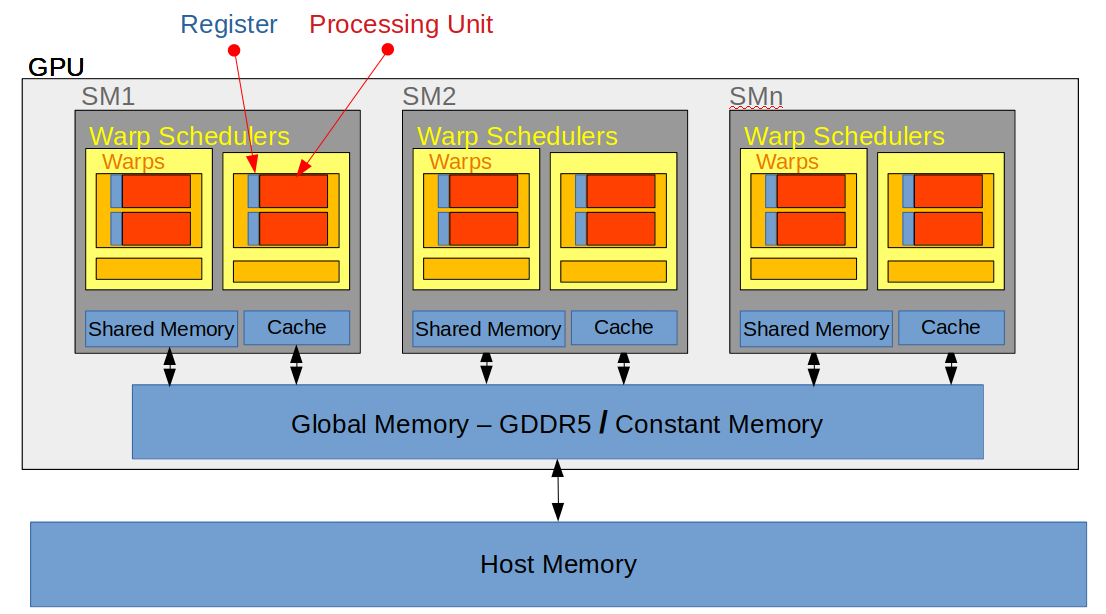
\includegraphics[width=\textwidth]{imgs/gpuArch.png}
	\caption[Figure]{Architecture of a GPU}
	\label{fig:gpuArch}
\end{figure}

\cite[Parallel Computing Book]{ParaComputation}

\section{Cores}
Figure \ref{fig:gpuArch} shows the architecture of a GPU. A modern GPU contains multiple so called streaming multiprocessors (SM). These work after the \gls{SIMD}. This means that there's only one instruction line that will be carried out by each processing unit. Special hardware indexers can identify the data on which this instruction operates for each processing unit individually. That's how it's possible to minimize chip-space by only having one instruction core but tons of data cores working on different junks of data.\\
Each processing unit contains at least 1 FPU, 1 int PU. It may also contain special function units, tensor calculation units, texture filtering unit etc. The Floating point unit can calculate 1 float operation per cycle. It needs multiple cycles to calculate doubles and can calculate even 2 16bit floats per cycle. Integer processing unit is build up similarly.\\
The streaming processor can work on multiple blocks. Those will be split into junks of 32 threads called warp. Those warps are put into a queue and wait for execution. The SM consists of multiple warp schedulers each consisting of 32 processing units that will work through the queue. Here it's important to mention that they don't work linearly through the actual set of threads. They just process the thread until a time consuming instruction like a load/store/branch starts. Then they switch to another set of 32 threads and continue at their actual instruction location. This is done because processing units are build up simple to minimize chip-space so they don't include stuff like branch prediction, pipe-lining etc. to work efficiently through time consuming instructions. Instead they rely on a how bunch of thread to compute in parallel to bypass such time consuming instruction.
Load/store to global memory are the longest instructions. They need about 100 Cycles to complete. This means we would need about 32*100=3200 threads to really fully utilize the all processing units while loading / storing data. 

\section{Memory}

There are 5 types of memory inside a GPU: Global Memory, Constant Memory, Shared Memory, Caches and Registers. Those can be seen in figure \ref{fig:gpuArch}. The first two of those can be written to by the host CPU with an API instruction (cudaMemcpy, cudaMemcpyToSymbol). To the later two there's only access from within the kernel. As Shared memory as well as caches are on chip memories they're very fast but cost also a lot of chip-space. Therefore it's a very limited resource. Registers are even faster than shared memory and cache because there directly embedded in the computing units. The constant memory can only be written to by the host controller but not by a kernel. The kernel has only read access. That's because everything that is stored inside the constant memory will be copied to the cache when the kernel launches which makes it very fast, but also limited in space.\\
The last memory is the global memory which is the biggest and by far the slowest one. Therefore it has a lot of potential to improve performance.\\

\subsection{Memory Parallelism}
As the access times for DDR is very long (multiple nanoseconds) it's build up is highly parallel to reach the bandwidth modern CPUs/GPUs demand. Figure \ref{fig:gpuChannels} shows a simplified DDR system. It's basic cell stores one bit of information via a capacitance. Multiple Cells are combined into a block and multiple blocks serves a channel. Each channel has it's own channel controller that is capable of issuing multiple data requests. Those requests are concurring IF they don't request data from the same block. This makes it possible to interleave data requests like it's shown in figure \ref{fig:gpuInterleave}.
\begin{figure}[H]
	\centering
	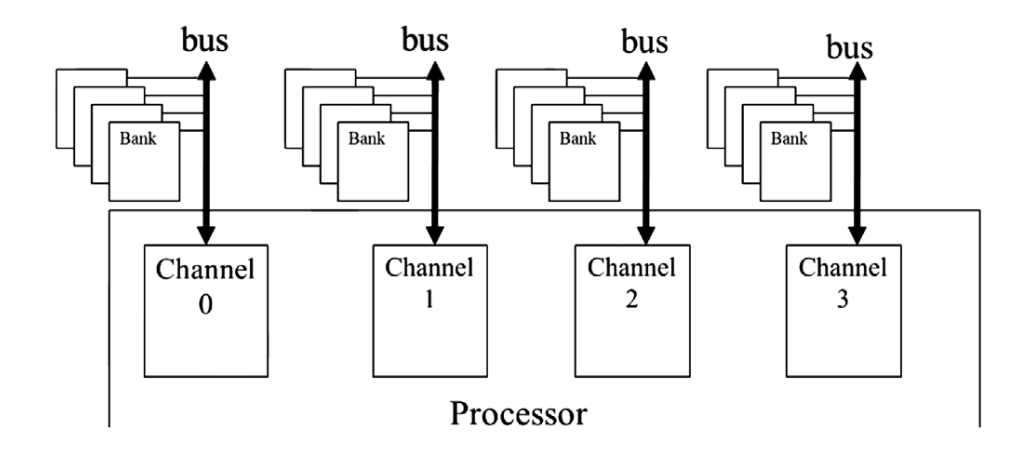
\includegraphics[width=\textwidth]{imgs/channeksbanks.png}
	\caption[Figure]{Architecture of GDDR5. \cite[Parallel Computing Book, p. 112]{ParaComputation}}
	\label{fig:gpuChannels}
\end{figure}
\begin{figure}[H]
	\centering
	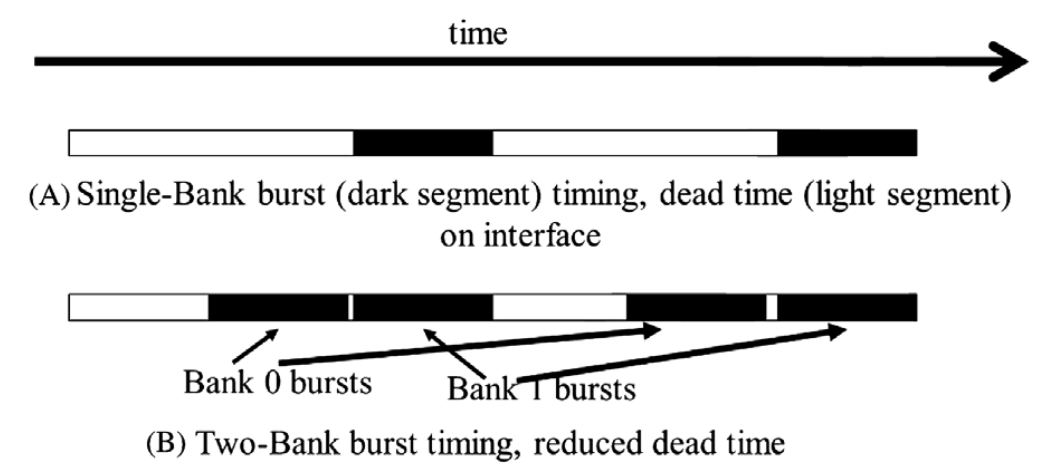
\includegraphics[width=\textwidth]{imgs/interleaveDDR.png}
	\caption[Figure]{Shows interleaved memory access.\cite[Parallel Computing Book, p. 113]{ParaComputation}}
	\label{fig:gpuInterleave}
\end{figure}

As this is done automatically the programmer must only ensure that enough thread simultaneously access the memory to utilize the whole bandwidth available. As the granularity of those blanks is very fine (128byts = 32floats) the max performance will be reached if the thread slots inside the streaming multiprocessors are utilized and a whole warp accesses data that is coalesced.\\

\subsection{Memory Coalescing}
Another important thing for accessing the global memory is to access grouped data as the device can access the global memory only in transactions of 32-, 64- or 128-bytes. Those bytes of one transaction are of sequencial memory locations (Example: N, N+1, N+2...N+64). Therefore if only one float value (4 bytes) is needed 3/4 of the transaction is wasted. Figure \ref{fig:gpuCoalescing} shows a good example for storing a matrix in the global memory. When accessing the data from the kernel in the order the data is stored, the maximum amount of coalescing is used.

\begin{figure}[H]
	\centering
	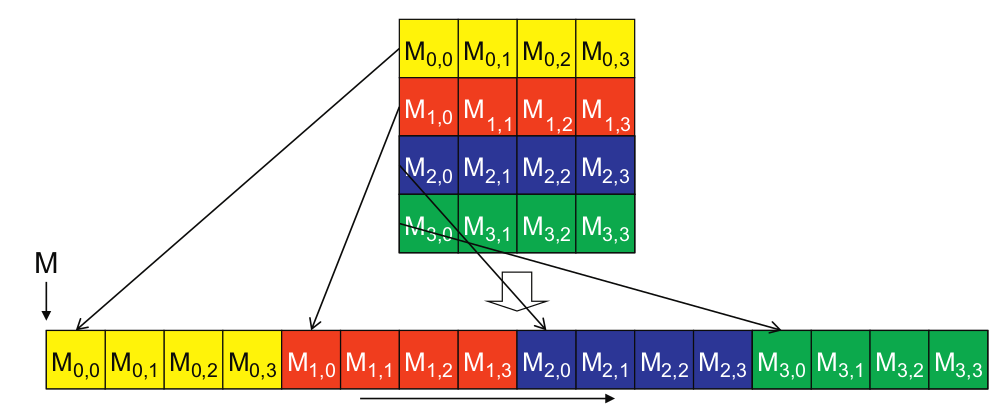
\includegraphics[width=0.6\textwidth]{imgs/coalecing.png}
	\caption[Figure]{Coalescing memory. \cite[Parallel Computing Book, p. 106]{ParaComputation}}
	\label{fig:gpuCoalescing}
\end{figure}

\subsection{Corner Tuning}
Corner Tuning is a method to access uncoalesced data in a coalesced way. This is done with using the shared memory. As access times don't differ in the shared memory for coalesced and uncoalesced data the solution is simply to copy the uncoalesced data in a coalesced way from the global memory to the shared memory and do the uncoalesced access there like it's shown in figure \ref{fig:gpuCornerTuning}

\begin{figure}[H]
	\centering
	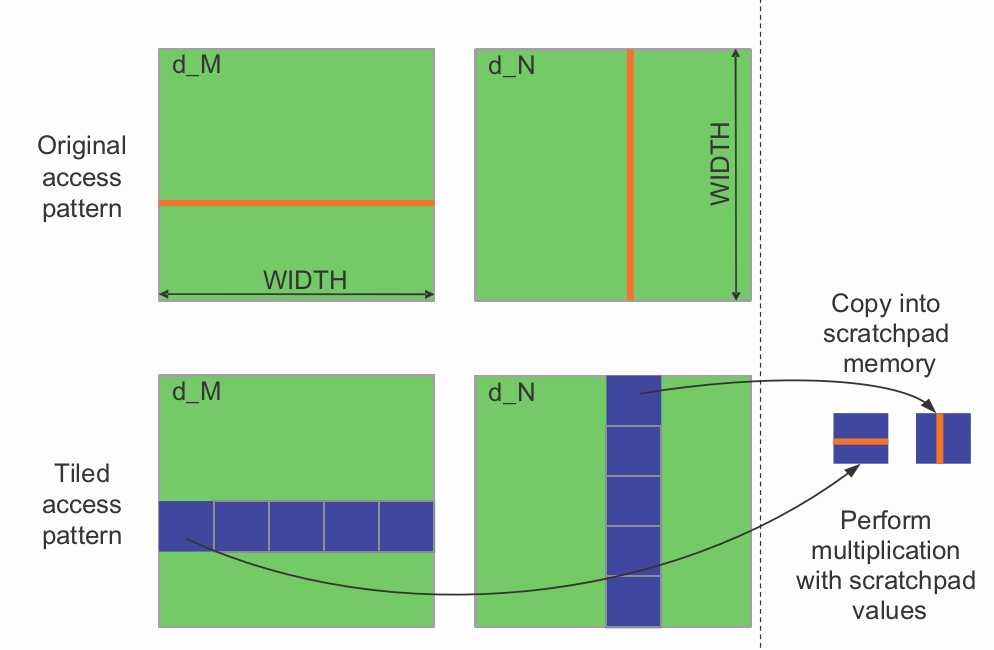
\includegraphics[width=0.7\textwidth]{imgs/cornerTuning.png}
	\caption[Figure]{Image shows corner tuning of uncoalesced data. \cite[Parallel Computing Book, p. 110]{ParaComputation}}
	\label{fig:gpuCornerTuning}
\end{figure}

\pagebreak

\section{Performance Considerations Overview}

The following checkpoints should be considered when optimizing an algorithm:
\begin{itemize}
	\item Are the resident threads of each SM nearly fully used?
	\item Isn't the number of threads reduced by the amount of registers used inside the kernel?
	\item Isn't the number of threads reduced by the amount of shared memory used be the kernel?
	\item Isn't the number of threads reduced by the max. number of blocks that can reside inside a SM?
	\item Are global memory accesses in coalesced bursts of at least 128 bytes.
	\item Are there enough parallel global memory accesses to fully utilize the global memory access bandwidth?
	\item Is Host-To-Device data transfer interleaved over several kernel calls to use the maximal PCI bandwidth?
	\item Did you use shared  / constant memory for global memory data that's accessed more than once? (Don't forget to corner tune your data)
	\item Did you maximize the compute-to-global-memory-access ratio? (Higher than 30 is good, higher than 50 is excellent.)
	\item Did you use caching effects as well as possible for similar data access that's not to the shared memory.
	\item Is the warp padding minimized?
	\item The most important performance aspect is to have a good, parallel algorithm.
\end{itemize}

This is just a list of points to give you an idea where to start and what to optimize.

